% Make appendix with alphabetical numbering:
\appendix
\renewcommand{\thesection}{\Alph{section}}
\subsection{Part 1: Mercury Spectrum}
\begin{figure}[H]
    \centering
    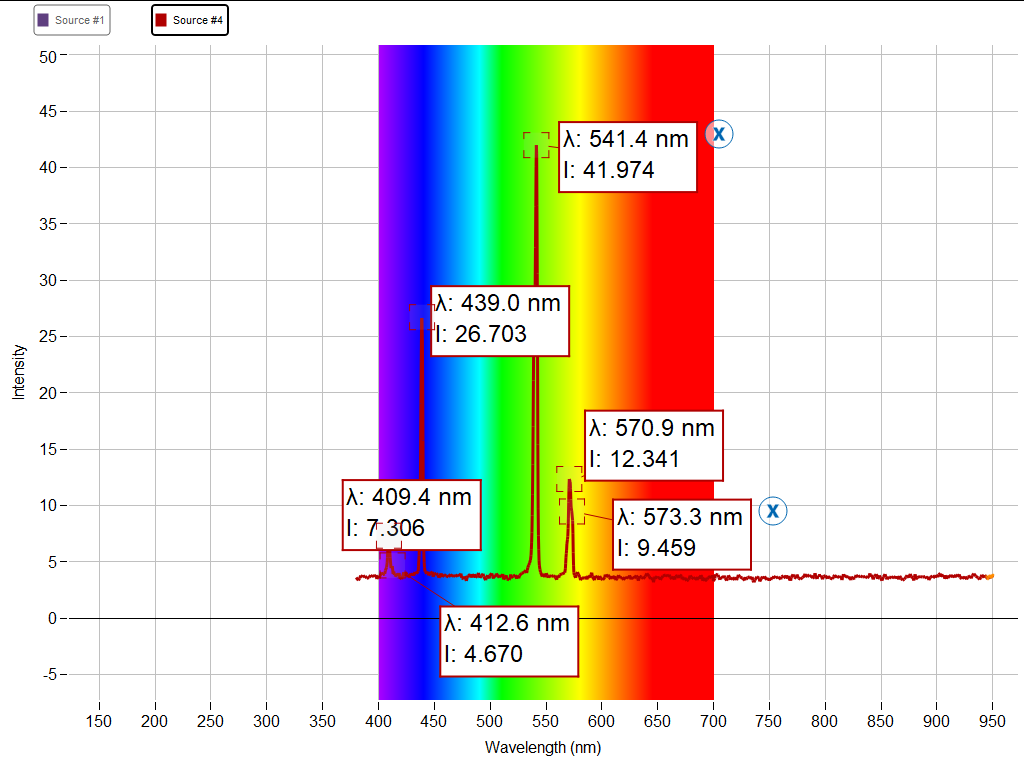
\includegraphics[width=0.8\textwidth]{Results/photospectrometry/mercury.png}
    \caption{Spectral Lines of Mercury}
    \label{fig:mercury_spectrum}
\end{figure}

\subsection{Part 2: Hydrogen Spectrum}
\begin{figure}[H]    \centering
    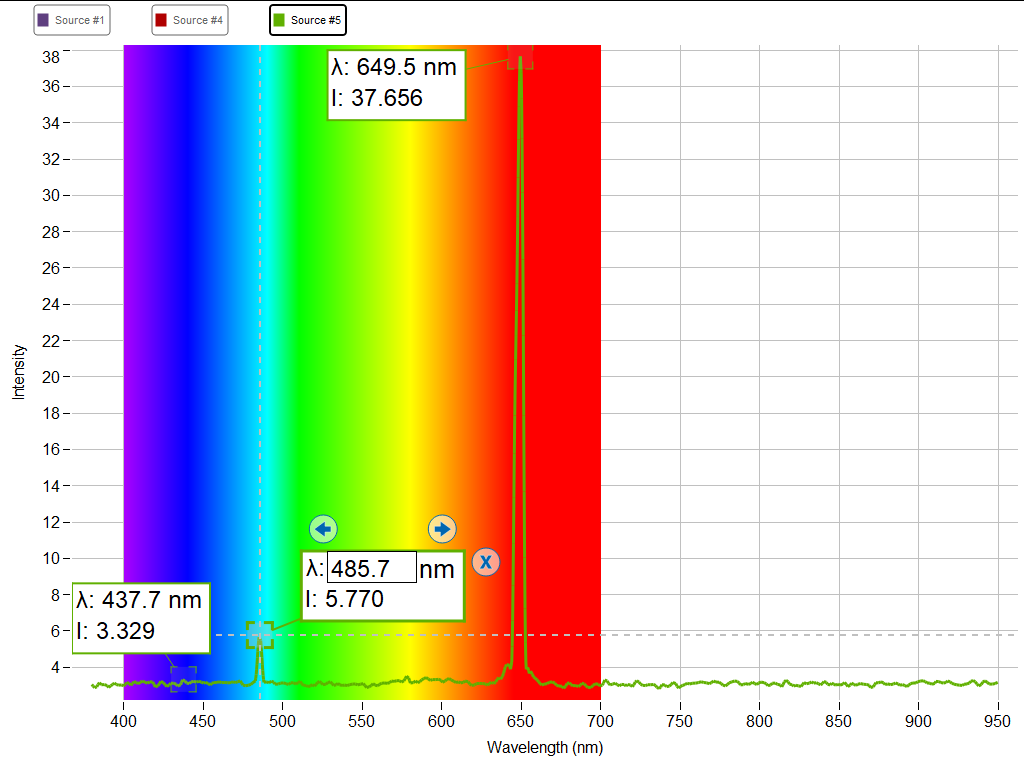
\includegraphics[width=0.8\textwidth]{Results/photospectrometry/hydrogen.png}
    \caption{Spectral Lines of Hydrogen}
    \label{fig:hydrogen_spectrum}
\end{figure}


% Calibration Function: \lambda = 1.068x - 32.78
\begin{table}[H]
    \centering
    % Table with 2 rows: measured \lambda and calibrated \lambda
    \begin{tabular}{|c|c|}
        \hline
        Measured Wavelength (nm) & Calibrated Wavelength (nm) \\
        \hline
        $437.7 \pm 3.14$ & $434.76 \pm 3.14$ \\
        $485.7 \pm 4.40$ & $486.04 \pm 4.40$ \\
        $649.5 \pm 5.66$ & $660.97 \pm 5.66$ \\
        \hline
    \end{tabular}
    \caption{Calibration of Hydrogen Spectrum}
\end{table}

\subsection{Part 3: Helium Spectrum}
\begin{figure}[H]    \centering
    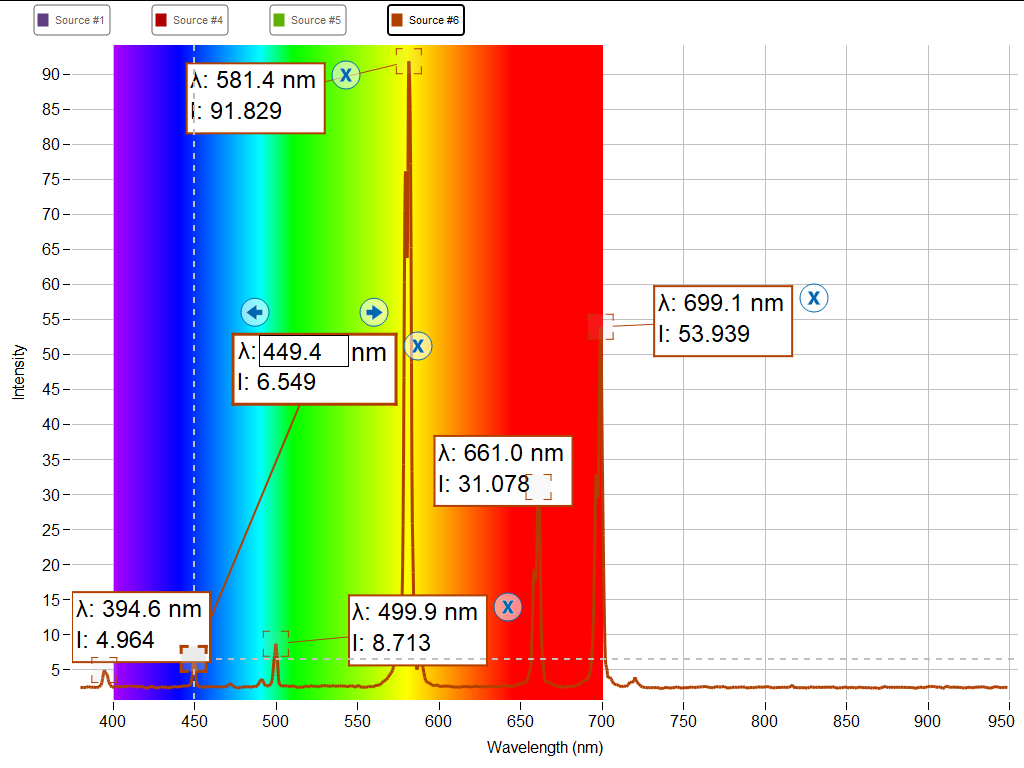
\includegraphics[width=0.8\textwidth]{Results/photospectrometry/helium.png}
    \caption{Spectral Lines of Helium}
    \label{fig:helium_spectrum}
\end{figure}

\begin{table}[H]
    \centering
    \begin{tabular}{|c|c|}
        \hline
        Measured Wavelength (nm) & Calibrated Wavelength (nm) \\
        \hline
        $394.60 \pm 4.30$ & $388.73 \pm 4.30$ \\
        $449.40 \pm 3.07$ & $447.26 \pm 3.07$ \\
        $499.90 \pm 3.68$ & $501.19 \pm 3.68$ \\
        $581.40 \pm 5.52$ & $588.24 \pm 5.52$ \\
        $661.00 \pm 5.52$ & $673.25 \pm 5.52$ \\
        $699.10 \pm 4.91$ & $713.94 \pm 4.91$ \\
        \hline
    \end{tabular}
    \caption{Calibration of Helium Spectrum}\end{table}

\subsection{Part 4: Unknown Spectrum}
\begin{figure}[H]    \centering
    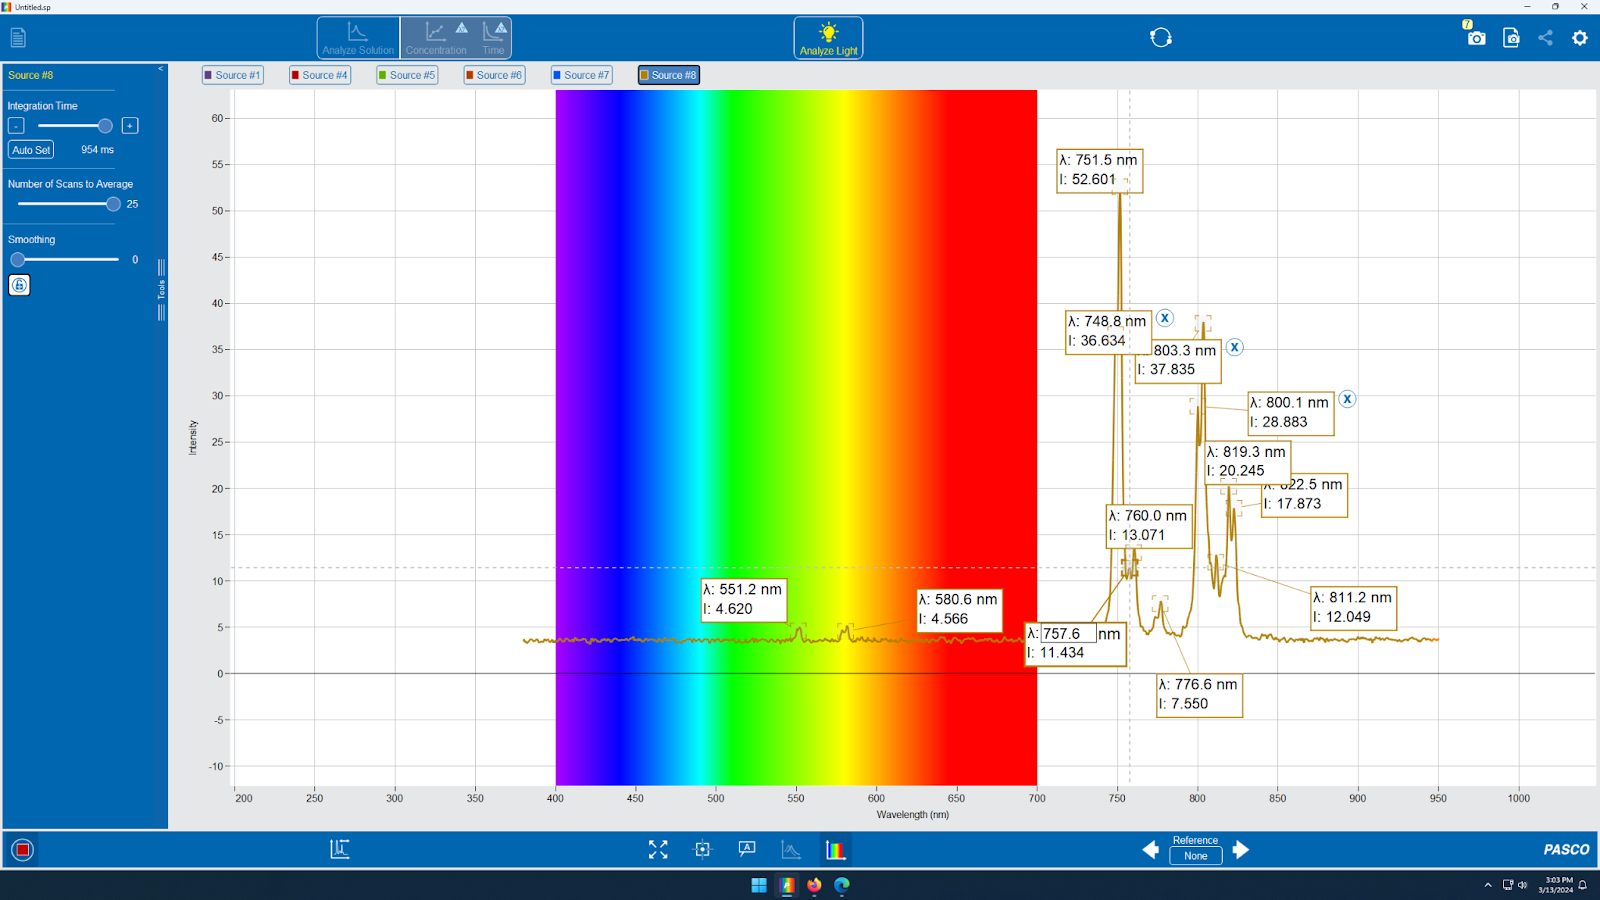
\includegraphics[width=0.8\textwidth]{Results/photospectrometry/unknown.png}
    \caption{Spectral Lines of Unknown Gas}
    \label{fig:unknown_spectrum}
\end{figure}

\begin{table}
    \centering
    \begin{tabular}{|c|c|}
        \hline
        Measured Wavelength (nm) & Calibrated Wavelength (nm) \\
        \hline
        $551.20 \pm 3.74$ & $555.98 \pm 3.74$ \\
        $580.60 \pm 5.60$ & $587.38 \pm 5.60$ \\
        $748.80 \pm 5.60$ & $767.02 \pm 5.60$ \\
        $751.50 \pm 5.60$ & $769.90 \pm 5.60$ \\
        $757.60 \pm 3.74$ & $776.42 \pm 3.74$ \\
        $760.00 \pm 3.74$ & $778.98 \pm 3.74$ \\
        $776.60 \pm 4.98$ & $796.71 \pm 4.98$ \\
        $800.10 \pm 7.47$ & $821.81 \pm 7.47$ \\
        $803.30 \pm 7.47$ & $825.22 \pm 7.47$ \\
        $811.20 \pm 4.36$ & $833.66 \pm 4.36$ \\
        $819.30 \pm 6.23$ & $842.31 \pm 6.23$ \\
        $822.50 \pm 6.23$ & $845.73 \pm 6.23$ \\
        \hline
    \end{tabular}
    \caption{Calibration of Unknown Spectrum}
\end{table}

\subsection{Part 5: Absorbance of Dyes}
\begin{figure}[H]    \centering
    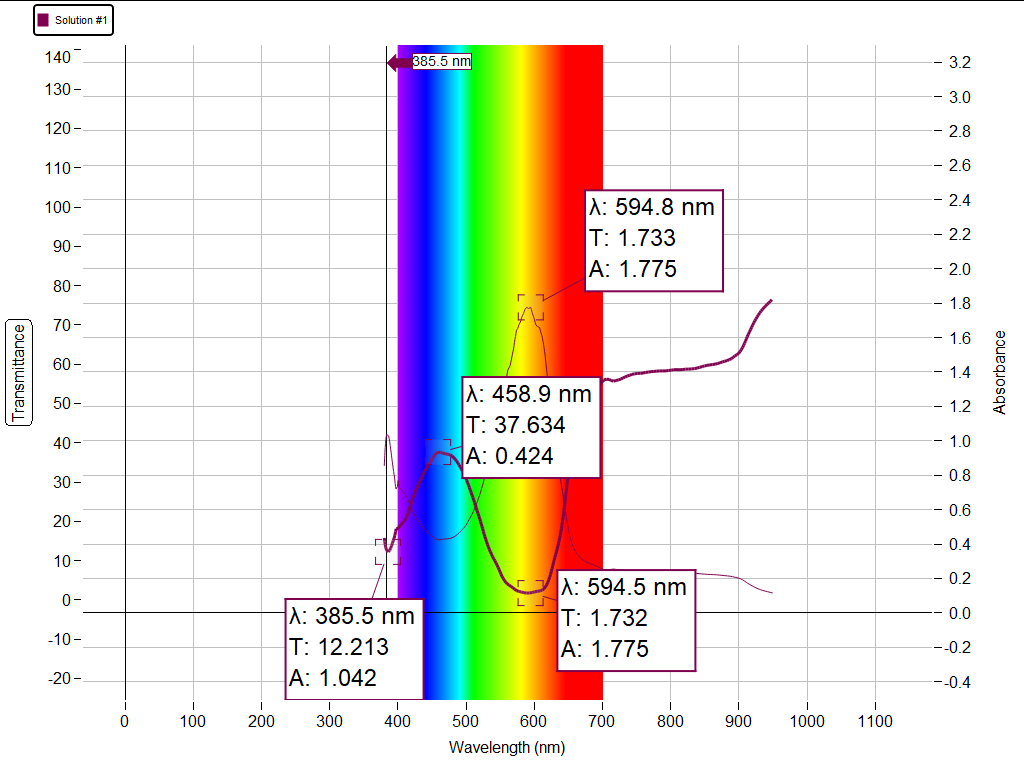
\includegraphics[width=0.8\textwidth]{Results/absorption_spectrometry/blue.png}
    \caption{Absorbance and transmittance of blue dye}
    \label{fig:blue_spectrum}
\end{figure}

\begin{figure}[H]    \centering
    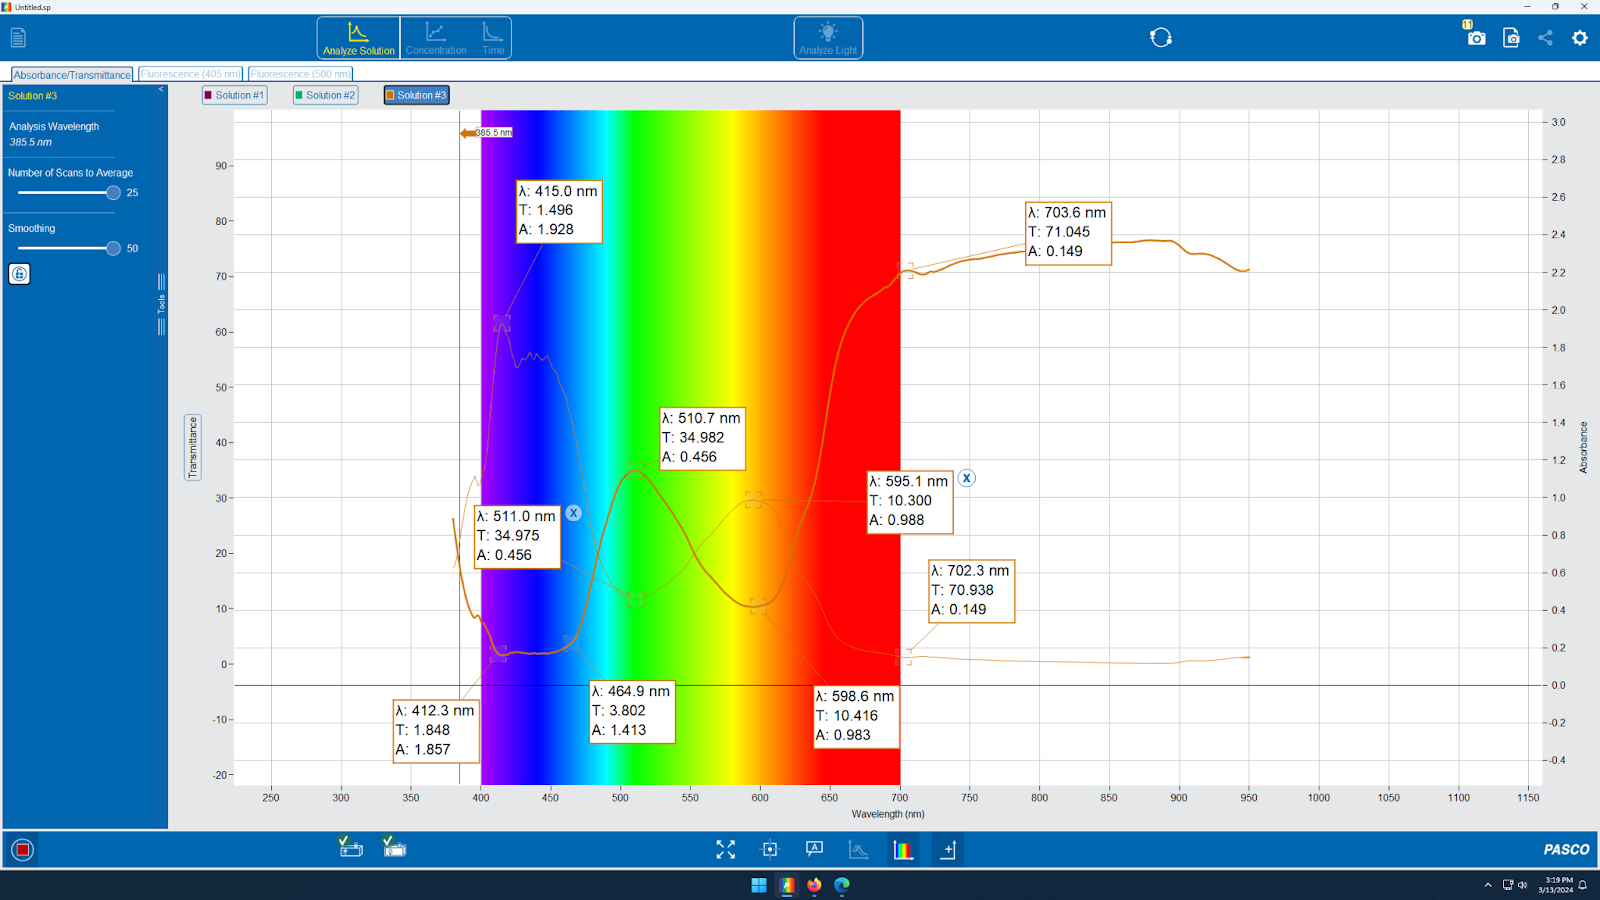
\includegraphics[width=0.8\textwidth]{Results/absorption_spectrometry/green.png}
    \caption{Absorbance and transmittance of green dye}
    \label{fig:green_spectrum}
\end{figure}

\subsection{Part 6: Fluorescence Spectrum}
\begin{figure}[H]    \centering
    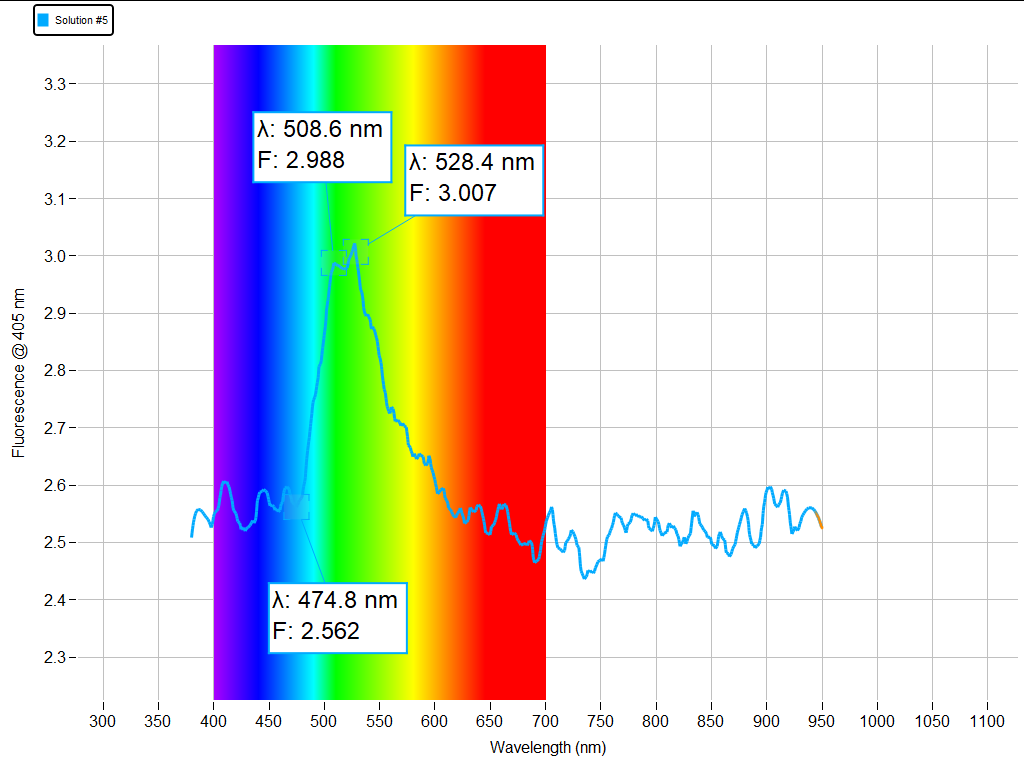
\includegraphics[width=0.8\textwidth]{Results/fluourescence_spectrometry/405nm.png}
    \caption{Fluorescence spectrum of yellow dye excited with 405nm light}
    \label{fig:fluorescence}
\end{figure}

\begin{figure}[H]    \centering
    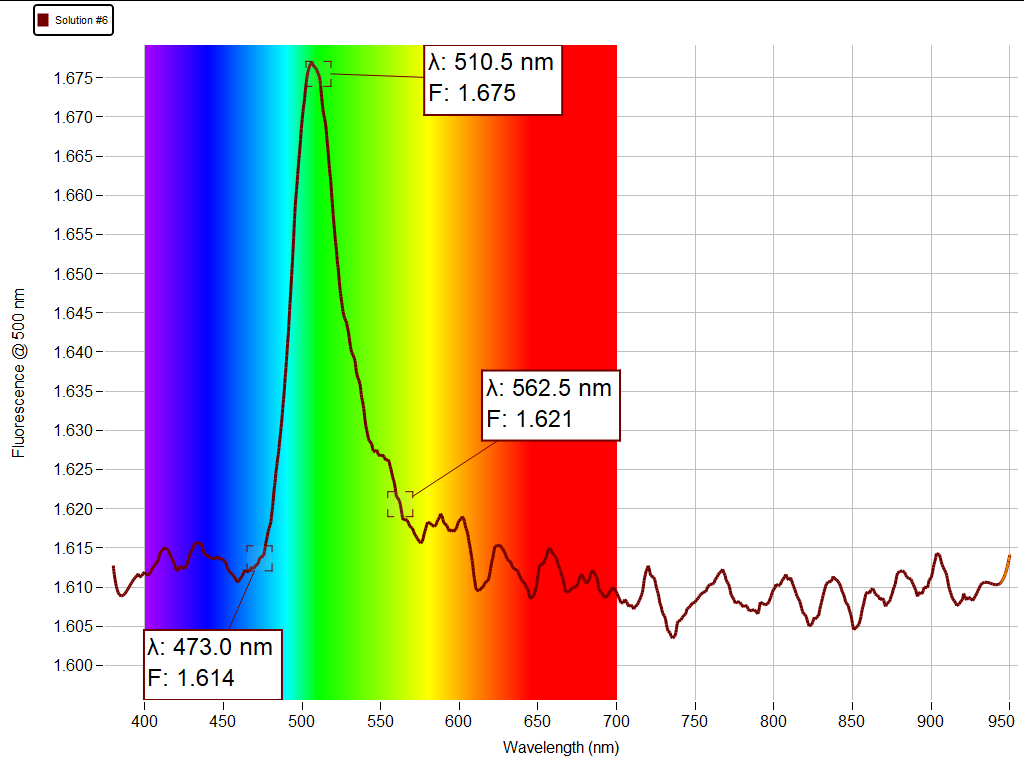
\includegraphics[width=0.8\textwidth]{Results/fluourescence_spectrometry/500nm.png}
    \caption{Fluorescence spectrum of yellow dye excited with 500nm light}
    \label{fig:fluorescence2}
\end{figure}